\section{Auswertung}
\label{sec:Auswertung}

%Siehe \autoref{fig:plot}!
\subsection{Berechnung der Landé-Faktoren}
\label{ssec:lande}

Für beide Resonanzstellen werden jeweils die Stromstärken für die Sweep-Spule $I_\text{s}$ und für die Horizontalspule $I_\text{h}$ in Abhängigkeit von der Frequenz $f$.
Mit dem Radius $R$ und der Windungszahl $N$ einer Spule kann über REF ZU HELMHOLTZ das Magentfeld $B$ aus den Stromstärken berechnet werden.
Die Abmessungen der drei Spulen sind 
\begin{align*}
    R_\text{sw} &= \qty{0.16390}{\meter} \\
    N_\text{sw} &= \qty{11}{} \\
    R_\text{hor} &= \qty{0.15790}{\meter} \\
    N_\text{hor} &= \qty{154}{} \\
    R_\text{ver} &= \qty{0.11735}{\meter} \\
    N_\text{ver} &= \qty{20}{}.
\end{align*}
In horizontaler Richtung werden die erzeugten Magnetfelder der Sweep-Spule und der horizontalen Spule addiert.
Die so berechnten Messwerte sind in \autoref{tab:f} notiert.

\begin{table}
    \centering
    \caption{Horizontale Magnetfelder an den Resonanzstellen von beiden Isotopen mit eingestellten Stromstärken der Spulen.}
    \label{tab:f}
    \begin{tabular}{r r r r r r r}
        \toprule
        $f \,/\, \unit{\kilo\hertz}$ & $I_\text{1,s} \,/\, \unit{\ampere}$ & $I_\text{1,h} \,/\, \unit{\ampere}$ & $B_\text{1} \,/\, \unit{\milli\tesla}$ & $I_\text{2,s} \,/\, \unit{\ampere}$ & $I_\text{2,h} \,/\, \unit{\ampere}$ & $B_\text{2} \,/\, \unit{\micro\tesla}$\\
        \midrule
        $100 $ & $625.0\pm1.0$ & $734.0\pm1.0$ & $0.0\pm3.0$ & $0.0\pm3.0$  & $37.7\pm2.6$ & $44.3\pm2.6$ \\
        $200 $ & $440.0\pm1.0$ & $677.0\pm1.0$ & $30.0\pm3.0$ & $30.0\pm3.0$  & $52.9\pm2.6$ & $67.2\pm2.6$ \\
        $300 $ & $422.0\pm1.0$ & $775.0\pm1.0$ & $48.0\pm3.0$ & $48.0\pm3.0$  & $67.6\pm2.6$ & $88.9\pm2.6$ \\
        $400 $ & $296.0\pm1.0$ & $770.0\pm1.0$ & $72.0\pm3.0$  & $72.0\pm3.0 $ & $81.0\pm2.6$ & $109.6\pm2.6$ \\
        $500 $ & $306.0\pm1.0$ & $898.0\pm1.0$ & $90.0\pm3.0$  & $90.0\pm3.0 $ & $97.4\pm2.6$ & $133.1\pm2.6$ \\
        $600 $ & $322.0\pm1.0$ & $710.0\pm1.0$ & $102.0\pm3.0$ & $126.0\pm3.0$ & $108.9\pm2.6$ & $153.3\pm2.6$ \\
        $700 $ & $334.0\pm1.0$ & $698.0\pm1.0$ & $120.0\pm3.0$ & $150.0\pm3.0$ & $125.4\pm2.6$ & $173.7\pm2.6$ \\
        $800 $ & $380.0\pm1.0$ & $432.0\pm1.0$ & $132.0\pm3.0$ & $192.0\pm3.0$ & $138.7\pm2.6$ & $194.4\pm2.6$ \\
        $900 $ & $607.0\pm1.0$ & $554.0\pm1.0$ & $132.0\pm3.0$ & $210.0\pm3.0$ & $152.4\pm2.6$ & $217.6\pm2.6$ \\
        $1000$ & $783.0\pm1.0$ & $710.0\pm1.0$ & $144.0\pm3.0$ & $222.0\pm3.0$ & $173.5\pm2.6$ & $237.5\pm2.6$ \\
        \bottomrule
    \end{tabular}
\end{table}

Die Beziehung zwischen dem Magnetfeld und der Frequenz ist linear, daher wird mittels eines Fits eine Gerade durch die Messwerte gelegt.
Dieser wird mit der Python Bibliothen Scipy durchgeführt.
Als Fit-Funktion wird dabei eine Gerade der Form
\begin{equation}
    B(f) = a \cdot f + b
\end{equation}
genutzt.
Das Ergenis dieses Fits ist in \autoref{fig:frequenz} dargestellt.
\begin{figure}
    \centering
    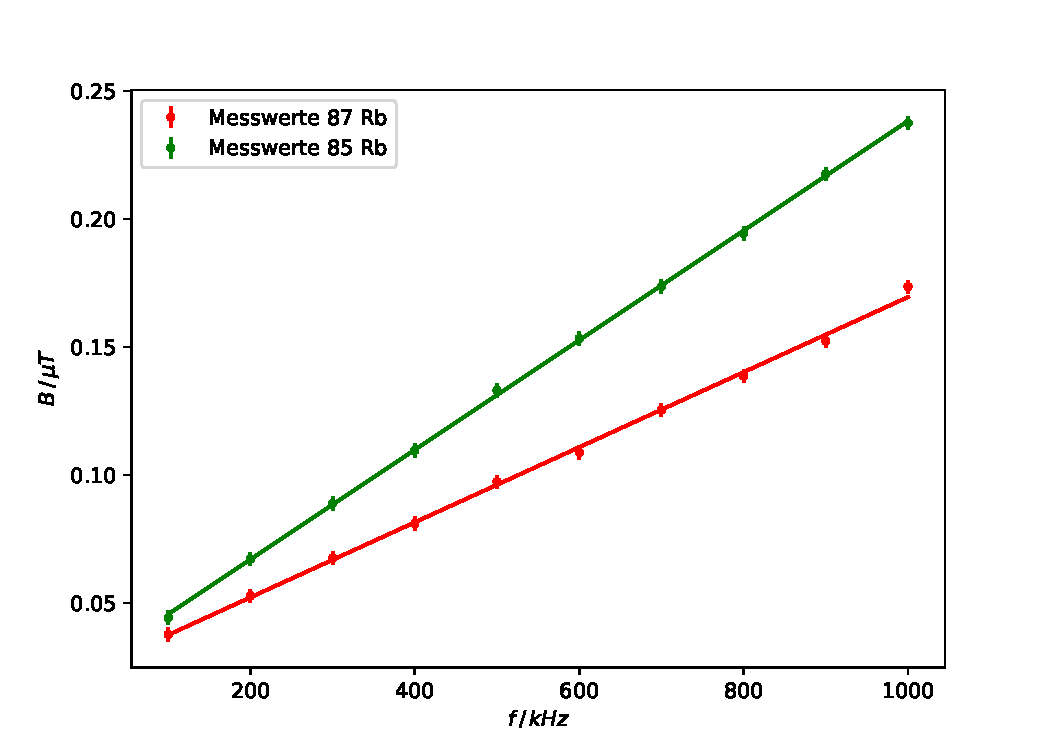
\includegraphics[width=0.8\textwidth]{plots/frequenz.pdf}
    \caption{Fit der Magnetfelder in Abhängigkeit der Frequenz zur Bestimmung der Landé-Faktoren.}
    \label{fig:frequenz}
\end{figure}
Die vom Fit bestimmten Parameter sind 
\begin{align*}
    a_\text{87} &= \qty{1.466(22)e-10}{\per\hertz} \\
    b_\text{87} &= \qty{2.29(13)e-05}{\tesla} \\
    a_\text{85} &= \qty{2.141(29)e-10}{\per\hertz} \\
    b_\text{85} &= \qty{2.42(18)e-05}{\tesla}.
\end{align*}
Wird REF ZUR ZEEMAN GLEICHUNG entsprechend umgestellt, ergibt sich der Zusammenhang
\begin{equation}
    g_\text{f} = \frac{m_\text{e}}{e \cdot a} \cdot 4\pi.
\end{equation}
Darüber wird der Landé-Faktor für beide Isotope 
\begin{align*}
    g_\text{f,87} &= \qty{0.487(7)}{} \\
    g_\text{f,85} &= \qty{0.334(5)}{}.
\end{align*}
bestimmt.


\begin{table}
    \centering
    \caption{Periodendauer der Rabi-Oszillationen in Abhängigkeit der RF-Amplitude für beide Peaks.}
    \label{tab:A}
    \begin{tabular}{r r r}
        \toprule
        $A \,/\, \unit{\volt}$ & $T_\text{1} \,/\, \unit{\milli\second}$ & $T_\text{2} \,/\, \unit{\milli\second}$\\
        \midrule
        $1.0 $ & $4.70 $ & $6.00 $\\
        $1.5 $ & $3.16 $ & $4.40 $\\
        $2.0 $ & $2.40 $ & $3.40 $\\
        $2.5 $ & $1.92 $ & $2.80 $\\
        $3.0 $ & $1.68 $ & $2.40 $\\
        $3.5 $ & $1.44 $ & $2.00 $\\
        $4.0 $ & $1.26 $ & $1.90 $\\
        $4.5 $ & $1.12 $ & $1.50 $\\
        $5.0 $ & $0.99 $ & $1.48 $\\
        $6.0 $ & $0.84 $ & $1.20 $\\
        $8.0 $ & $0.60 $ & $0.88 $\\
        $10.0$ & $ 0.47$ & $0.72 $\\
        \bottomrule
    \end{tabular}
\end{table}